% Volume II: Calculus, Analysis, and Continuous Mathematics
% Continuity note for Chapter 12.
% Previous dependencies: Chapter 2's typed function notation; Chapter 3's vector spaces, norms, inner products, angles, and orthogonality; Chapter 4's linear maps and matrices; Chapter 5's projection geometry; Chapter 6's eigenvectors and spectral directions; Chapter 8's derivatives and integrals; Chapter 9's derivative-as-linear-map viewpoint; Chapter 11's densities, integration, and change-of-variables discipline.
% New durable concepts: function spaces; pointwise versus norm-based comparison; L^2 inner products and norms; orthogonal families of functions; basis coefficients; Hilbert-space intuition; linear operators on functions; kernel and convolution operators; differential and integral operators; eigenfunctions; Fourier series; Fourier transform; spectra; convolution theorem; sampling; Nyquist rate; aliasing; frequency response; low-pass and anti-alias filters.
% Forward hooks: Later chapters reuse function spaces for stochastic processes, kernels, Gaussian processes, variational objectives, and function-valued parameters; operators for PDEs, neural fields, recurrent dynamics, and convolutional networks; Fourier methods for signal processing, spectral regularization, receptive fields, image models, and experimental time-series analysis.
% Notation commitments: Time or one-dimensional input is t; functions are f,g,h; intervals are [a,b] or [0,T]; the real L^2 inner product is <f,g>=\int f(t)g(t)\,dt, with complex conjugation <f,g>=\int f(t)\overline{g(t)}\,dt when needed; operators are T:V\to W; kernel operators use (Tf)(t)=\int K(t,s)f(s)\,ds; convolution uses (h*f)(t)=\int h(t-s)f(s)\,ds; Fourier-series coefficients are c_k; Fourier transforms use \widehat f(\omega)=\int f(t)e^{-i\omega t}\,dt and f(t)=(1/2\pi)\int \widehat f(\omega)e^{i\omega t}\,d\omega; sampling uses x[n]=x(n\Delta t) and f_s=1/\Delta t.
% Figure plan: four ImageGen raster figures under imagegen-figures/ch12-* are referenced: function-space geometry for 12.1; operators, kernels, linearity, and eigenfunctions for 12.2; Fourier modes and spectra for 12.3; sampling, aliasing, Nyquist, and anti-alias filters for 12.4.
\section{Chapter 12: Function Spaces, Operators, and Fourier Analysis}
\label{ch:function-spaces-operators-fourier-analysis}

Earlier chapters built geometry for finite lists of numbers. A vector could be a point, an arrow, a row of data, a parameter vector, or a neural population activity pattern. A matrix could transform such vectors, project them, or reveal preferred directions. Chapters 8--11 then added calculus and integration, so we can now measure changes and accumulated quantities over continuous domains. Chapter 12 extends the same geometric language from finite vectors to functions.

The central move is simple but powerful: treat a whole signal \(f(t)\) as one mathematical object. A function can have a length, an angle with another function, coordinates in a basis, and transformations applied to it. The transformations are operators. Fourier analysis is the most important example of this viewpoint: it chooses sinusoidal basis functions and rewrites signals by frequency.

\paragraph{Chapter problem.}
How can functions be treated as vectors, how can transformations of functions be treated as linear maps, and how do Fourier methods turn signals, filters, and sampling into geometry?

\paragraph{Section map.}
Section 12.1 defines spaces of functions, especially \(L^2\), where inner products and norms compare entire signals. Section 12.2 defines linear operators on functions and shows how derivative, integral, kernel, convolution, and projection operators fit the matrix analogy. Section 12.3 develops Fourier series and the Fourier transform as orthogonal coordinates in frequency. Section 12.4 explains sampling, aliasing, Nyquist's criterion, and filters.

\subsection{12.1 Spaces of functions}

\paragraph{Motivating question.}
If a function is not just a formula but an entire signal, what does it mean for two functions to be close, perpendicular, or represented by coordinates?

\paragraph{Beginner setup.}
A \emph{function space} is a collection of functions that is treated as a geometric space. Instead of comparing two numbers or two finite vectors, we compare two whole curves. For example, let
\[
f(t)=t,\qquad g(t)=t^2,\qquad 0\leq t\leq 1.
\]
Both functions live in a space of square-integrable functions on \([0,1]\). Their difference is another function,
\[
(f-g)(t)=t-t^2.
\]
A natural distance between them is the \(L^2\) distance:
\[
\|f-g\|_2
=\left(\int_0^1 |f(t)-g(t)|^2\,dt\right)^{1/2}.
\]
This is the continuous analogue of the Euclidean distance between two long sampled vectors.

Function spaces solve the problem of comparing and transforming objects with infinitely many possible input values. A neural voltage trace, an audio waveform, an image intensity field, a tuning curve, and a probability density are not single numbers. But once they live in a suitable function space, we can ask familiar geometric questions: What is their norm? What is their inner product? Which basis functions explain most of them? Which operator transforms them?

What to keep in mind: a function space is not "all possible formulas." It is a typed collection with rules. The interval, integrability assumptions, boundary conditions, and notion of equality all matter. In \(L^2\), two functions that differ only on a set of measure zero are treated as the same object because integrals cannot detect isolated point changes.

\begin{figure}[htbp]
\centering
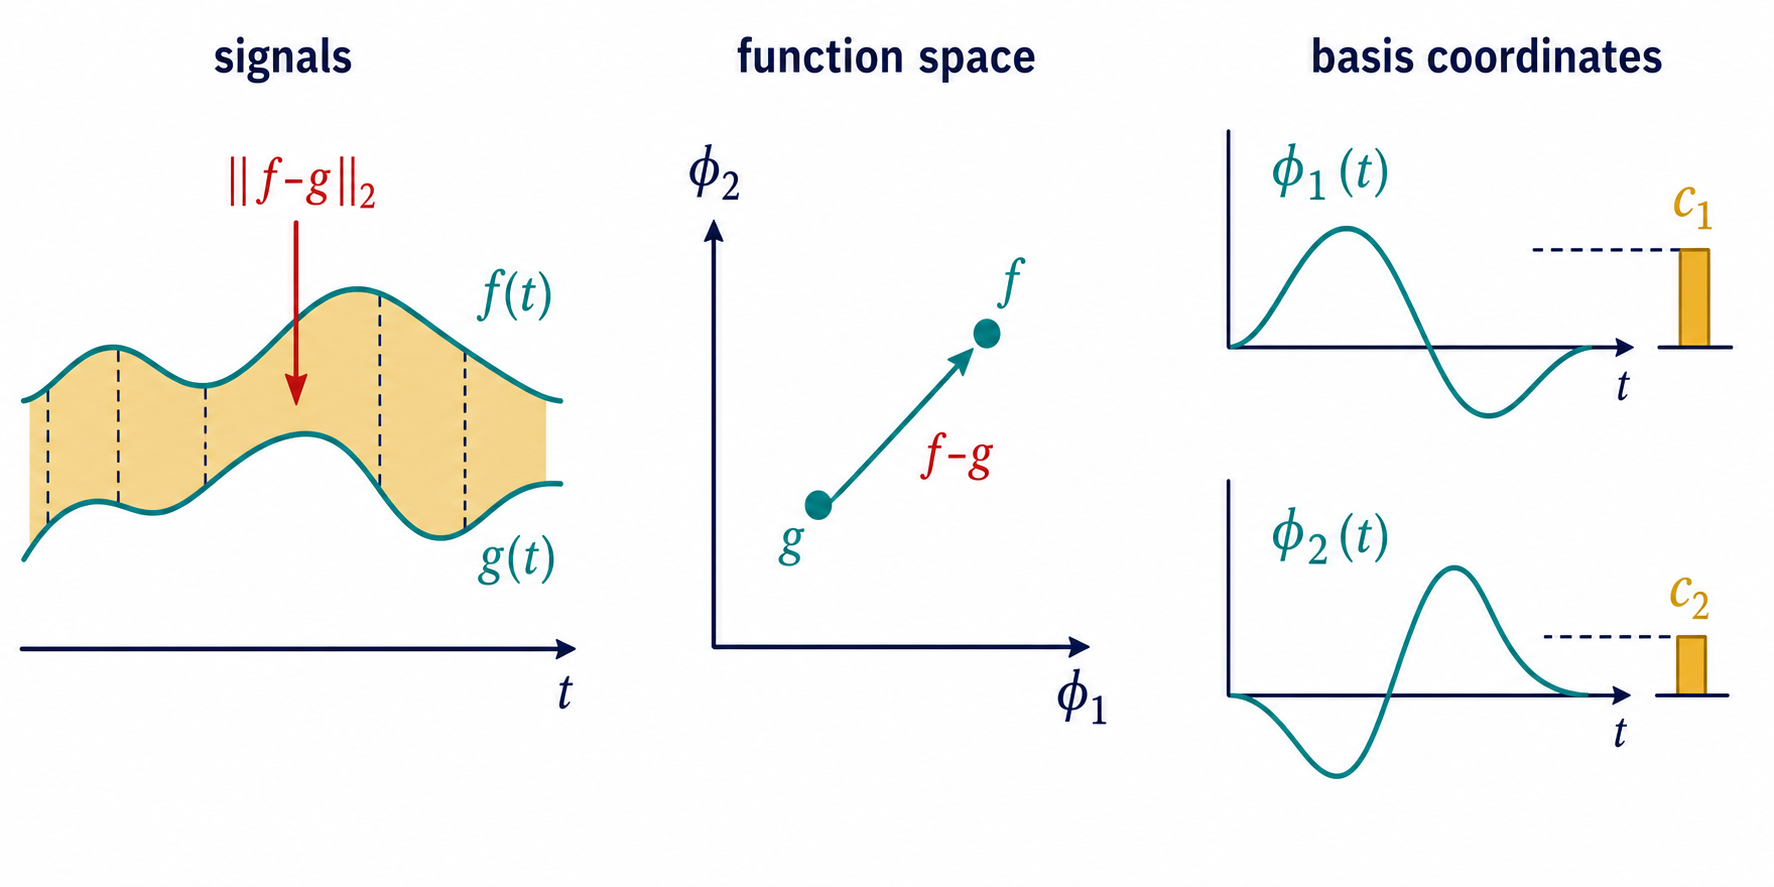
\includegraphics[width=0.96\linewidth]{imagegen-figures/ch12-function-spaces.png}
\caption{Functions can be treated as vector-like objects. The \(L^2\) distance \(\|f-g\|_2\) measures the accumulated squared difference between two curves. In an abstract function space, \(f\) and \(g\) are points and \(f-g\) is their displacement. Choosing basis functions \(\phi_1,\phi_2,\ldots\) gives coordinate coefficients such as \(c_1,c_2\).}
\label{fig:ch12-function-spaces}
\end{figure}

\paragraph{Formal setup.}
Let \(I=[a,b]\) be an interval. The vector space \(C(I)\) consists of continuous real-valued functions \(f:I\to\mathbb{R}\). The space \(L^2(I)\) is built from measurable functions whose squared magnitude has finite integral:
\[
L^2(I)=\left\{f:I\to\mathbb{R}:\int_I |f(t)|^2\,dt<\infty\right\},
\]
with the important formal convention that functions equal almost everywhere are treated as the same \(L^2\) element. In other words, an \(L^2\) object is really an equivalence class of functions modulo changes on measure-zero sets. This is why changing a function at one isolated time point does not change its \(L^2\) norm or distance.
For real-valued functions in \(L^2(I)\), define
\[
\langle f,g\rangle
=\int_I f(t)g(t)\,dt,
\qquad
\|f\|_2
=\sqrt{\langle f,f\rangle}.
\]
For complex-valued functions, the inner product is usually
\[
\langle f,g\rangle
=\int_I f(t)\overline{g(t)}\,dt,
\]
so that \(\langle f,f\rangle\geq 0\); the complex \(L^2\) space replaces \(\mathbb{R}\) by \(\mathbb{C}\) in the same equivalence-class setup. The central equation for this section is the \(L^2\) norm:
\[
\boxed{\|f\|_2^2=\int_I |f(t)|^2\,dt.}
\]
It says that the length of a function is accumulated energy over the domain. With this norm and inner product, \(L^2(I)\) is complete: every Cauchy sequence of \(L^2\) functions has a limit in \(L^2(I)\). A complete inner-product space is called a Hilbert space, so \(L^2(I)\) is the main Hilbert-space example for this chapter.

A family \(\{\phi_k\}\) is \emph{orthonormal} if
\[
\langle \phi_j,\phi_k\rangle
=
\begin{cases}
1, & j=k,\\
0, & j\neq k.
\end{cases}
\]
When a function can be represented in an orthonormal basis, its coordinates are inner products:
\[
c_k=\langle f,\phi_k\rangle,
\qquad
f\approx \sum_{k=1}^m c_k\phi_k.
\]

\paragraph{Core intuition.}
Figure~\ref{fig:ch12-function-spaces} shows three views of the same idea. In the left panel, two curves differ over time; the \(L^2\) distance accumulates that discrepancy across the whole interval. In the middle panel, the functions are points in an abstract space, just as vectors were points in Chapter 3. In the right panel, basis functions act like coordinate axes. Coefficients tell us how much of each basis direction is present.

The analogy with finite-dimensional vectors is strong but not perfect. If a signal is sampled at \(n\) time points, it becomes a vector in \(\mathbb{R}^n\). As the sampling gets denser, sums such as
\[
\sum_{i=1}^n f(t_i)g(t_i)\Delta t
\]
approach integrals such as \(\int f(t)g(t)\,dt\). Function-space inner products are therefore continuous versions of dot products. But infinite-dimensional spaces also bring new issues: convergence, boundary behavior, and whether an operator is stable on the chosen space. The completeness of \(L^2\) is what makes limits of energy-convergent approximations stay inside the space, rather than falling out of the mathematical setting.

Common misconceptions are worth separating. First, pointwise closeness and \(L^2\) closeness are different. Two functions can disagree at one point and still have zero \(L^2\) distance. Second, a function space is not chosen after the calculation; it is part of the problem statement. A derivative operator needs differentiable functions, while a Fourier transform needs integrability or square-integrability assumptions. Third, basis functions are not decorative curve shapes. They are coordinate directions in a space of functions.

This section reuses vector-space language from Chapter 3 and projection language from Chapter 5. It prepares operators in Section 12.2, Fourier bases in Section 12.3, and kernels, Gaussian processes, neural fields, and function-valued optimization objectives in later chapters.

\paragraph{Main theorem: Cauchy-Schwarz in \(L^2\).}
For real- or complex-valued \(f,g\in L^2(I)\), using the complex inner-product convention above when needed,
\[
|\langle f,g\rangle|
\leq
\|f\|_2\|g\|_2.
\]
Therefore the \(L^2\) inner product defines a legitimate angle-like similarity measure between functions.

\emph{Proof sketch.}
If \(g=0\), the result is immediate. Otherwise, consider the nonnegative quantity
\[
0\leq \|f-\alpha g\|_2^2
=\langle f-\alpha g,f-\alpha g\rangle
\]
for any scalar \(\alpha\). Expanding the inner product, using the convention \(\langle f,g\rangle=\int f\overline{g}\), gives
\[
\|f-\alpha g\|_2^2
=\|f\|_2^2-\overline{\alpha}\langle f,g\rangle-\alpha\langle g,f\rangle+|\alpha|^2\|g\|_2^2.
\]
Choose
\[
\alpha=\frac{\langle f,g\rangle}{\|g\|_2^2}.
\]
Because \(\langle g,f\rangle=\overline{\langle f,g\rangle}\), substituting this value leaves
\[
0\leq \|f\|_2^2-\frac{|\langle f,g\rangle|^2}{\|g\|_2^2}.
\]
Rearranging gives
\[
|\langle f,g\rangle|^2\leq \|f\|_2^2\|g\|_2^2.
\]
Taking square roots proves the claim. For real-valued functions, this reduces to the familiar real quadratic proof. The mechanism is the same as in finite-dimensional vector geometry: the best scalar multiple of \(g\) cannot make a squared distance negative.

\paragraph{Worked examples.}
\emph{Small numerical example.} Let \(f(t)=t\) and \(g(t)=t^2\) on \([0,1]\). Then
\[
\langle f,g\rangle
=\int_0^1 t^3\,dt
=\frac14.
\]
Their norms are
\[
\|f\|_2
=\left(\int_0^1 t^2\,dt\right)^{1/2}
=\frac{1}{\sqrt{3}},
\qquad
\|g\|_2
=\left(\int_0^1 t^4\,dt\right)^{1/2}
=\frac{1}{\sqrt{5}}.
\]
Their squared distance is
\[
\|f-g\|_2^2
=\int_0^1 (t-t^2)^2\,dt
=\int_0^1(t^2-2t^3+t^4)\,dt
=\frac13-\frac12+\frac15
=\frac{1}{30}.
\]
Thus \(\|f-g\|_2=1/\sqrt{30}\).

\emph{ML/neuroscience example.} Suppose \(r_1(t)\) and \(r_2(t)\) are smoothed firing-rate responses of the same neuron to two stimuli over a one-second window. The quantity
\[
\|r_1-r_2\|_2
=\left(\int_0^1 |r_1(t)-r_2(t)|^2\,dt\right)^{1/2}
\]
measures how different the entire response time courses are, not just their peak rates. If a model represents each response by coefficients in basis functions \(\phi_k(t)\), then those coefficients become features for decoding stimulus identity.

\paragraph{ML/DL/neuroscience connections.}
In machine learning, a kernel method may compare inputs by first mapping each input to a function and then taking inner products in a function space. In deep learning, continuous signals are often discretized into vectors, but the operations they approximate -- smoothing, convolution, differentiation, and spectral filtering -- are naturally operators on functions. In neuroscience, spike trains are often smoothed into rate functions, local field potentials are time-varying functions, and tuning curves are functions from stimulus variables to response rates. The function \(f(t)\) becomes a signal, \(\|f\|_2^2\) becomes signal energy, and \(\langle f,g\rangle\) becomes overlap or similarity between response patterns.

\paragraph{Exercises.}
\begin{enumerate}[label=\textbf{12.1.\arabic*.}, leftmargin=*]
\item \textbf{Mechanical.} On \([0,1]\), compute \(\|f\|_2\) for \(f(t)=1-t\).
\item \textbf{Proof or derivation.} Show that if \(\langle f,g\rangle=0\), then \(\|f+g\|_2^2=\|f\|_2^2+\|g\|_2^2\). Interpret this as the Pythagorean theorem for functions.
\item \textbf{Numerical/computational.} Approximate \(\langle f,g\rangle\) for \(f(t)=\sin(\pi t)\) and \(g(t)=t\) on \([0,1]\) using the left-endpoint Riemann sum \(\sum_i f(t_i)g(t_i)\Delta t\) with \(t_i=i/4\), \(i=0,1,2,3\), and \(\Delta t=1/4\).
\item \textbf{Interpretation.} Two firing-rate curves have the same average firing rate but a large \(L^2\) distance. What does that say about their temporal structure?
\item \textbf{Debug the misconception.} A student says, "If two functions differ at one time point, they must be far apart in \(L^2\)." Explain why this is false and state what kind of difference \(L^2\) distance measures.
\end{enumerate}

\subsection{12.2 Linear operators}

\paragraph{Motivating question.}
What is the function-space analogue of a matrix, and how can we tell whether a transformation of signals is linear?

\paragraph{Beginner setup.}
An \emph{operator} is a map whose inputs and outputs are functions. A matrix \(A:\mathbb{R}^n\to\mathbb{R}^m\) takes a vector and returns a vector. A function operator \(T:V\to W\) takes a function \(f\in V\) and returns another function \(Tf\in W\). For example,
\[
(Df)(t)=f'(t)
\]
is a derivative operator on differentiable functions, and
\[
(If)(t)=\int_0^t f(s)\,ds
\]
is an integral operator.

The smallest nontrivial test is linearity. An operator \(T\) is linear if it preserves weighted sums:
\[
T(af+bg)=aT(f)+bT(g).
\]
This is exactly the same rule a matrix obeys. If \(f\) and \(g\) are signals and \(a,b\) are gains, a linear operator processes the mixed signal \(af+bg\) by producing the same mixture of the processed signals.

Operators solve the problem of describing transformations of whole functions: smoothing a noisy trace, differentiating a signal, delaying a waveform, projecting onto a basis, convolving with a receptive field, or evolving an initial condition through a dynamical system.

What to keep in mind: an operator is not automatically linear. Squaring a signal, rectifying it with a ReLU, normalizing it by its maximum, or thresholding it usually breaks linearity. Also, the domain matters. The derivative operator is not defined on arbitrary \(L^2\) functions; it needs additional smoothness or a weak-derivative interpretation.

\begin{figure}[htbp]
\centering
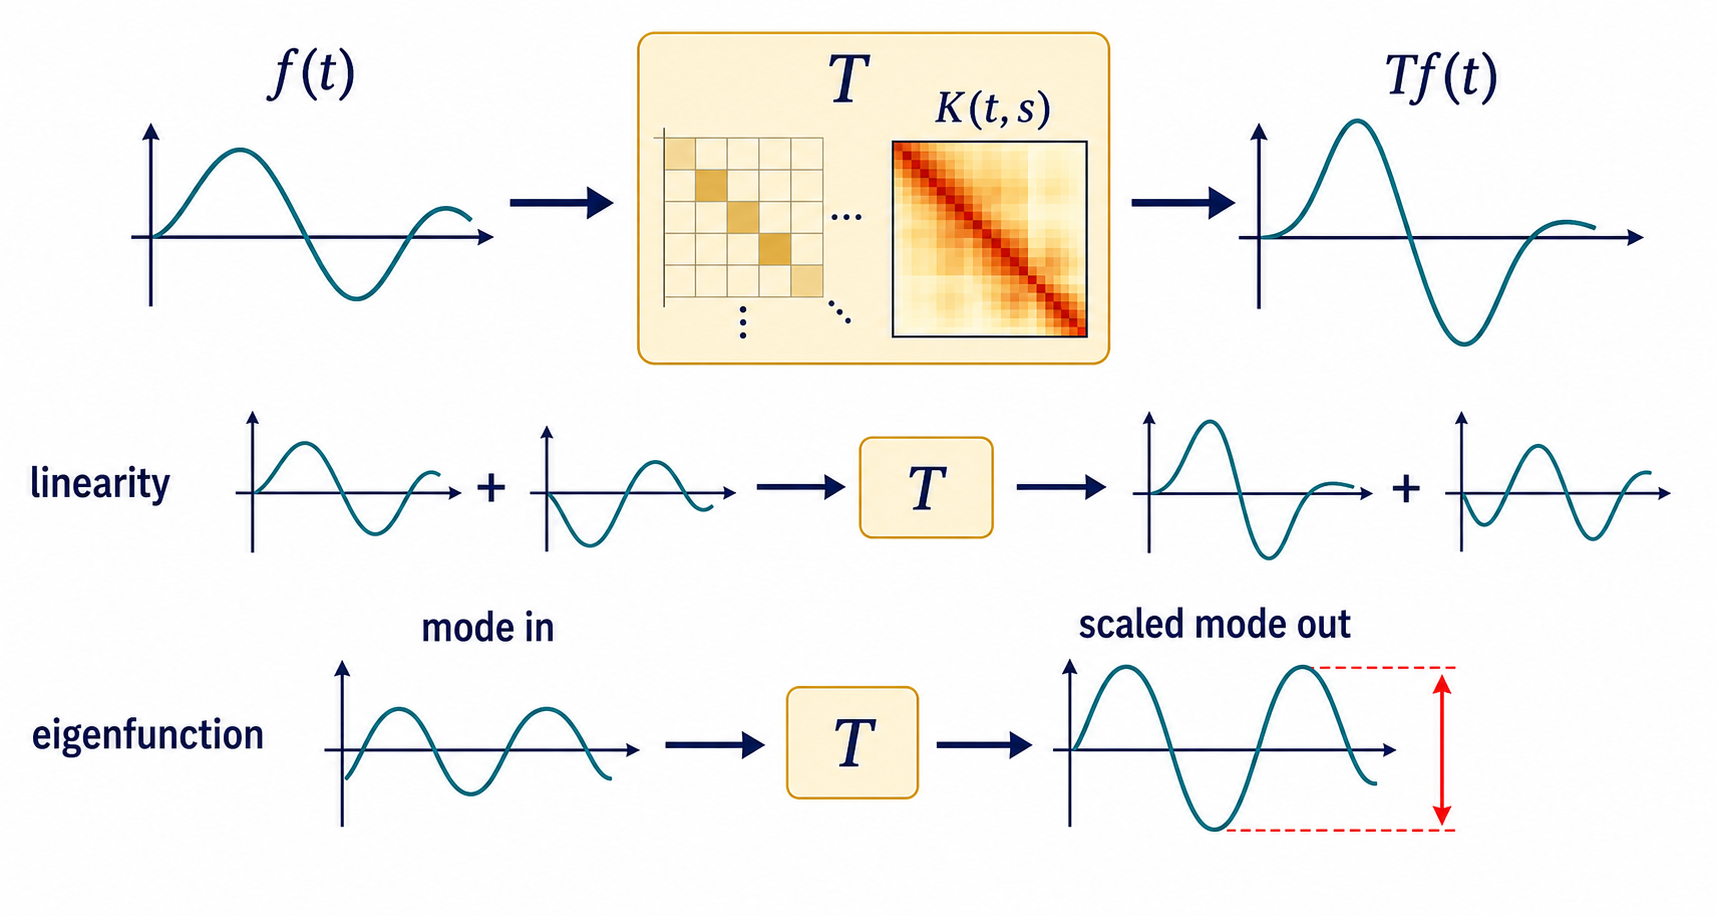
\includegraphics[width=0.96\linewidth]{imagegen-figures/ch12-linear-operators.png}
\caption{A linear operator maps an input function \(f(t)\) to an output function \((Tf)(t)\), much as a matrix maps an input vector to an output vector. Some operators are described by kernels \(K(t,s)\). Linearity means that processing a sum gives the sum of processed signals. An eigenfunction is a mode whose shape is preserved by the operator, up to a scalar factor.}
\label{fig:ch12-linear-operators}
\end{figure}

\paragraph{Formal setup.}
Let \(V\) and \(W\) be vector spaces of functions over the same scalar field, usually \(\mathbb{R}\) or \(\mathbb{C}\). An operator is a map
\[
T:V\to W.
\]
It is linear if, for all \(f,g\in V\) and all scalars \(a,b\),
\[
\boxed{T(af+bg)=aT(f)+bT(g).}
\]
Important examples include:
\[
(Df)(t)=f'(t),
\qquad
(If)(t)=\int_a^t f(s)\,ds,
\]
\[
(M_qf)(t)=q(t)f(t),
\qquad
(P_Uf)=\text{the projection of }f\text{ onto a subspace }U,
\]
and kernel operators
\[
(Tf)(t)=\int K(t,s)f(s)\,ds.
\]
A convolution operator is a special kernel operator:
\[
(h*f)(t)=\int_{-\infty}^{\infty} h(t-s)f(s)\,ds.
\]
Here \(h\) is the impulse response or filter kernel, and suitable integrability assumptions are required so the integral exists.

If \(V\) has a norm, an operator is \emph{bounded} if there is a constant \(C\) such that
\[
\|Tf\|_W\leq C\|f\|_V
\quad\text{for all }f\in V.
\]
Boundedness is the function-space version of stability: small input in the chosen norm cannot produce arbitrarily large output.

\paragraph{Core intuition.}
Figure~\ref{fig:ch12-linear-operators} shows the matrix analogy. A finite matrix stores numbers \(A_{ij}\) that say how input coordinate \(j\) contributes to output coordinate \(i\). A kernel \(K(t,s)\) plays a similar role: it says how input value \(f(s)\) contributes to output value \((Tf)(t)\). The integral sums all source locations \(s\), just as matrix multiplication sums over columns.

Derivative and convolution operators also show why eigenfunctions matter. A matrix eigenvector leaves the output direction unchanged. An operator eigenfunction leaves the output shape unchanged:
\[
T\phi=\lambda\phi.
\]
For many shift-invariant operators, sinusoids or complex exponentials are eigenfunctions. This is one reason Fourier analysis is so useful: it chooses basis functions that many signal-processing operators handle independently by frequency.

Common misconceptions parallel matrix misconceptions. First, an operator is not a formula with a letter \(T\); it is a typed map with a domain and codomain. Second, linearity is not the same as "having a straight graph." The operator \(D\) is linear even though it acts on nonlinear functions such as \(t^2\). Third, convolution is linear in the input \(f\) when the kernel \(h\) is fixed; if the kernel changes as a nonlinear function of \(f\), the overall transformation may not be linear.

This section directly extends Chapter 4's matrix-as-linear-map viewpoint. It prepares Fourier diagonalization of filters, PDE operators, kernel methods, recurrent linear systems, and convolutional neural networks.

\paragraph{Main derivation: kernel operators are linear.}
Let
\[
(Tf)(t)=\int K(t,s)f(s)\,ds
\]
for functions where the integral is well defined. For \(f,g\in V\) and scalars \(a,b\),
\[
T(af+bg)(t)
=\int K(t,s)\bigl(af(s)+bg(s)\bigr)\,ds.
\]
Using linearity of multiplication and integration,
\[
T(af+bg)(t)
=a\int K(t,s)f(s)\,ds
+b\int K(t,s)g(s)\,ds.
\]
Therefore
\[
T(af+bg)(t)
=a(Tf)(t)+b(Tg)(t).
\]
Because this holds for every output location \(t\), we have
\[
T(af+bg)=aT(f)+bT(g).
\]
The mechanism is the same as matrix multiplication: each output coordinate is a linear weighted sum of input values.

\paragraph{Worked examples.}
\emph{Small symbolic example.} Define
\[
(Tf)(t)=f'(t)+2f(t)
\]
on differentiable functions. If \(f(t)=t^2\), then
\[
(Tf)(t)=2t+2t^2.
\]
If \(g(t)=\sin t\), then
\[
(Tg)(t)=\cos t+2\sin t.
\]
For scalars \(a,b\),
\[
T(af+bg)(t)
=(af+bg)'(t)+2(af+bg)(t)
=a(f'(t)+2f(t))+b(g'(t)+2g(t)),
\]
so \(T\) is linear.

\emph{ML/neuroscience example.} A one-dimensional convolutional layer before its nonlinearity applies
\[
y_i=\sum_j h_j x_{i-j}
\]
to a discrete signal \(x\). This is a finite-dimensional version of the convolution operator
\[
(h*f)(t)=\int h(t-s)f(s)\,ds.
\]
The signal \(f\) becomes an input trace, the kernel \(h\) becomes a learned receptive field, and the output \(h*f\) is the filtered signal. The convolution step is linear in \(f\) when \(h\) is fixed; the full neural network layer becomes nonlinear only after adding bias terms and pointwise nonlinearities.

\paragraph{ML/DL/neuroscience connections.}
In machine learning, a kernel smoother is an operator that maps noisy data to a smoother function. In Gaussian process regression, covariance kernels define linear operations on function spaces. In deep learning, convolutional layers, attention with fixed weights, and linear recurrent dynamics are operator-like transformations of sequences or fields. In neuroscience, a receptive field maps a stimulus function to a predicted response by integration, and a neural field model applies spatial operators to activity functions over cortex. The operator \(T\) becomes a filter, synaptic connectivity map, differential equation generator, or learned linear layer.

\paragraph{Exercises.}
\begin{enumerate}[label=\textbf{12.2.\arabic*.}, leftmargin=*]
\item \textbf{Mechanical.} Let \((Tf)(t)=\int_0^t f(s)\,ds\). Compute \(Tf\) for \(f(t)=1+t\).
\item \textbf{Proof or derivation.} Prove directly from the definition that the derivative operator \(D f=f'\) is linear on the space of differentiable functions.
\item \textbf{Numerical/computational.} For the discrete convolution \(y_i=x_i+2x_{i-1}\) with missing indices treated as zero, compute \(y\) for \(x=(1,0,3,2)\).
\item \textbf{Interpretation.} In a receptive-field model \(r(t)=\int K(t,s)u(s)\,ds\), what are the input function, kernel, operator, and output function?
\item \textbf{Debug the misconception.} A student says, "The operator \(T(f)=f^2\) is linear because it sends functions to functions." Find \(T(f+g)\) and compare it with \(Tf+Tg\).
\end{enumerate}

\subsection{12.3 Fourier series and Fourier transform}

\paragraph{Motivating question.}
How can a signal be represented by frequency coordinates, and why do sinusoids form the natural basis for many operators?

\paragraph{Beginner setup.}
Fourier analysis expresses functions using sinusoidal building blocks. For a periodic signal on an interval of length \(T\), the basic modes are waves with frequencies \(k/T\), where \(k\) is an integer. A simple real example is
\[
x(t)=3+2\cos t-\sin(2t).
\]
This signal is already written as a sum of a constant mode, a frequency-1 cosine mode, and a frequency-2 sine mode. Fourier analysis answers the inverse question: given the signal \(x(t)\), how much of each sine and cosine mode is present?

The concept solves a coordinate problem. In the time domain, we see the signal's value at each time. In the frequency domain, we see which rhythms or spatial scales compose the signal. This is useful because many operators treat different frequencies in simple ways. Smoothing suppresses high frequencies. Differentiation amplifies high frequencies. Translation changes phase. Convolution multiplies spectra.

What to keep in mind: Fourier series and Fourier transforms are related but not identical. Fourier series handle periodic functions using discrete frequency indices. Fourier transforms handle nonperiodic functions on the real line using a continuous frequency variable. Both are changes of coordinates in a function space.

\begin{figure}[htbp]
\centering
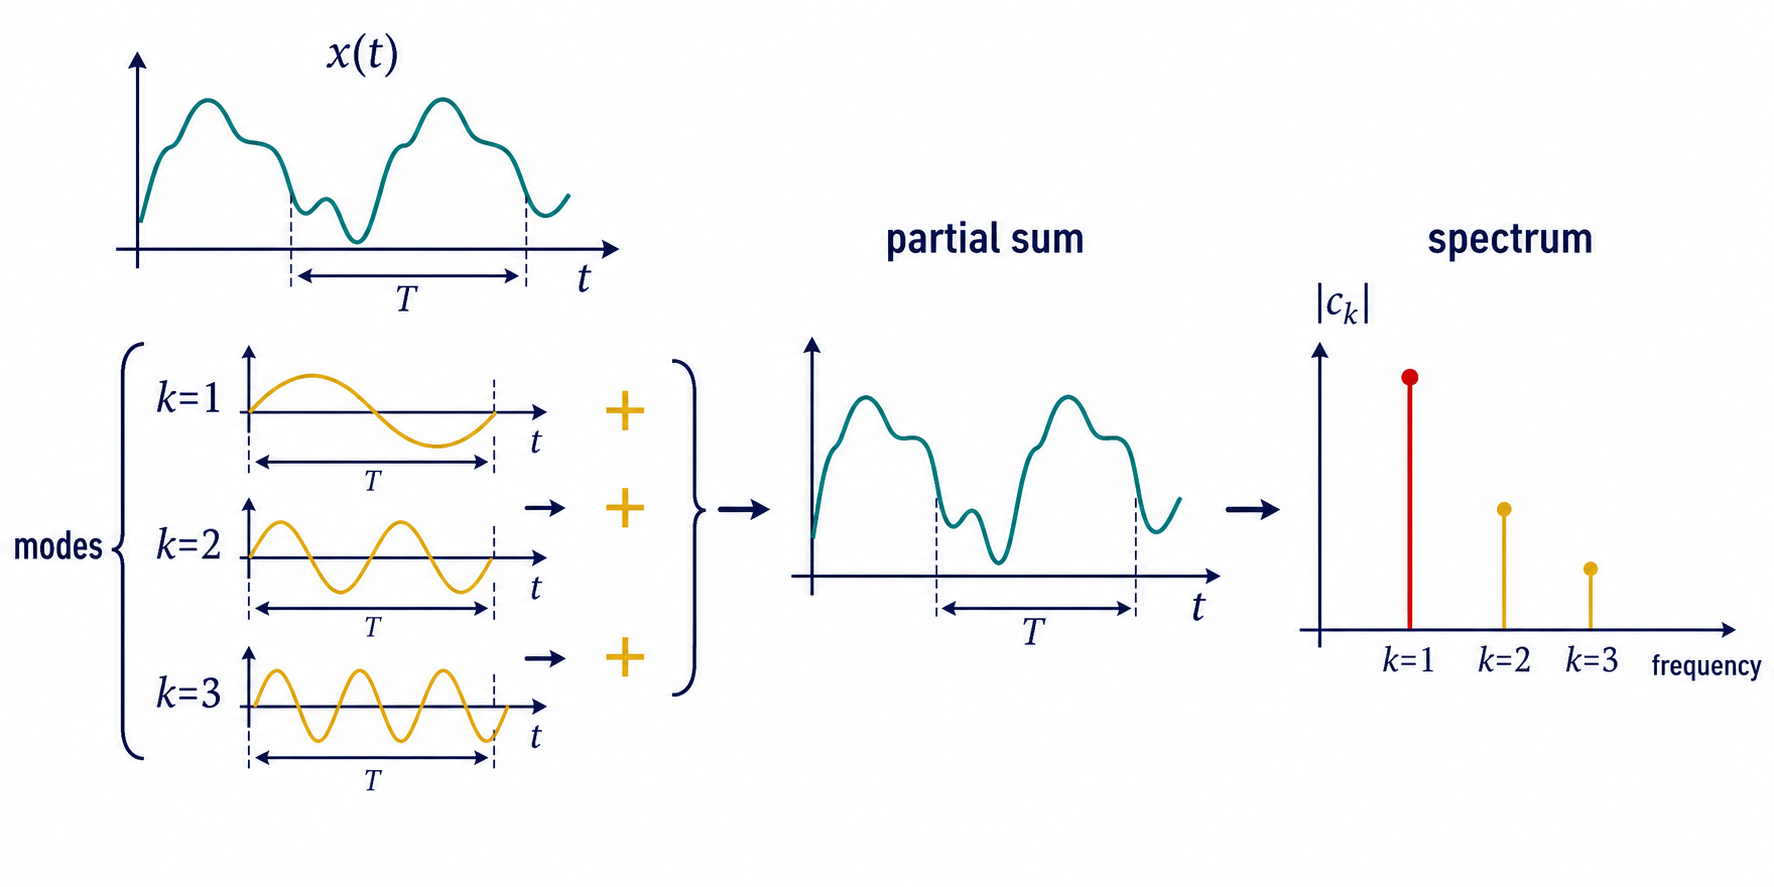
\includegraphics[width=0.96\linewidth]{imagegen-figures/ch12-fourier-decomposition.png}
\caption{Fourier analysis represents a signal by sinusoidal modes. A periodic signal \(x(t)\) can be approximated by a partial sum of modes \(k=1,2,3,\ldots\). The spectrum records the coefficient magnitude \(|c_k|\), showing which frequency coordinates are large.}
\label{fig:ch12-fourier-decomposition}
\end{figure}

\paragraph{Formal setup.}
For complex Fourier series on \([0,T]\), define
\[
\phi_k(t)=e^{i2\pi kt/T},
\qquad k\in\mathbb{Z}.
\]
These modes are orthogonal:
\[
\frac{1}{T}\int_0^T \phi_j(t)\overline{\phi_k(t)}\,dt
=
\begin{cases}
1, & j=k,\\
0, & j\neq k.
\end{cases}
\]
For a sufficiently nice periodic function \(f\), the Fourier coefficients are
\[
\boxed{
c_k=\frac{1}{T}\int_0^T f(t)e^{-i2\pi kt/T}\,dt
}
\]
and the Fourier series is
\[
f(t)\sim \sum_{k=-\infty}^{\infty} c_k e^{i2\pi kt/T}.
\]
For \(L^2\) functions, the series converges in energy. With additional smoothness, convergence can be pointwise except at jumps, where the series converges to the midpoint of the one-sided limits.

For nonperiodic signals on the real line, one common Fourier transform convention is
\[
\widehat f(\omega)
=\int_{-\infty}^{\infty} f(t)e^{-i\omega t}\,dt,
\]
with inverse transform
\[
f(t)
=\frac{1}{2\pi}\int_{-\infty}^{\infty}\widehat f(\omega)e^{i\omega t}\,d\omega.
\]
Different fields place constants differently; the convention must be stated.

\paragraph{Core intuition.}
Figure~\ref{fig:ch12-fourier-decomposition} should look familiar from earlier vector chapters. A vector \(v\) can be represented by coordinates along basis vectors. A periodic function \(f\) can be represented by coordinates along sinusoidal basis functions. The coefficient \(c_k\) is an inner product with the \(k\)th mode, so it measures overlap with that frequency.

The word "frequency" is not mysterious. A low-frequency sine wave changes slowly; a high-frequency sine wave oscillates rapidly. Sharp edges, abrupt jumps, and fine spatial details need high-frequency content. Smooth broad trends mostly use low frequencies. A spectrum is a coordinate plot showing how much of each frequency is present.

Fourier modes are especially important because they are eigenfunctions of shift-invariant linear operators. For example,
\[
\frac{d}{dt}e^{i\omega t}=i\omega e^{i\omega t}.
\]
The derivative changes only the coefficient, not the mode shape. Convolution behaves similarly:
\[
\widehat{h*f}(\omega)=\widehat h(\omega)\widehat f(\omega),
\]
under suitable integrability assumptions. This is the convolution theorem. It says that filtering in time becomes multiplication in frequency.

Common misconceptions include treating the Fourier transform as a new signal rather than a new coordinate description, ignoring normalization conventions, and assuming that a large high-frequency coefficient is always noise. High frequencies may be noise, but they may also be edges, spike timing, sharp stimulus changes, or meaningful oscillatory structure.

This section reuses orthogonality and projection from Chapters 3 and 5, eigenfunction ideas from Chapter 6, and integration from Chapter 11. It prepares spectral filters, signal processing, PDE solution methods, kernels, convolutional networks, and neural oscillation analysis.

\paragraph{Main derivation: Fourier coefficients from orthogonality.}
Assume a periodic function has an expansion
\[
f(t)=\sum_{k=-\infty}^{\infty} c_k e^{i2\pi kt/T}
\]
and that termwise integration is justified. To isolate coefficient \(c_m\), multiply both sides by \(e^{-i2\pi mt/T}\) and integrate over one period:
\[
\int_0^T f(t)e^{-i2\pi mt/T}\,dt
=
\sum_k c_k\int_0^T e^{i2\pi kt/T}e^{-i2\pi mt/T}\,dt.
\]
Combine the exponentials:
\[
\int_0^T e^{i2\pi(k-m)t/T}\,dt
=
\begin{cases}
T, & k=m,\\
0, & k\neq m.
\end{cases}
\]
All terms vanish except the \(k=m\) term, leaving
\[
\int_0^T f(t)e^{-i2\pi mt/T}\,dt
=Tc_m.
\]
Therefore
\[
c_m=\frac{1}{T}\int_0^T f(t)e^{-i2\pi mt/T}\,dt.
\]
The algebra is exactly the coordinate extraction rule from an orthonormal basis: take an inner product with the basis direction you want.

\paragraph{Worked examples.}
\emph{Small symbolic example.} On \([0,2\pi]\), let
\[
f(t)=3+2\cos t-\sin(2t).
\]
In real Fourier form, the average value is \(3\), the coefficient of \(\cos t\) is \(2\), and the coefficient of \(\sin(2t)\) is \(-1\). All other sine and cosine coefficients are zero. The spectrum has energy at frequency \(0\), frequency \(1\), and frequency \(2\). The negative sign on \(\sin(2t)\) is phase information; the magnitude tells how strongly that mode is present.

\emph{ML/neuroscience example.} Suppose \(x(t)\) is a local field potential recorded during a task. A Fourier transform produces \(\widehat x(\omega)\), whose magnitude indicates how strongly different oscillation frequencies appear in the recording. If a band-pass filter keeps \(8\)--\(12\) Hz content, then the operator is selecting a frequency band. In a convolutional neural network for audio, a learned filter also has a frequency response: the learned kernel \(h\) transforms input spectra by multiplying them by \(\widehat h(\omega)\).

\paragraph{ML/DL/neuroscience connections.}
In machine learning, Fourier features map inputs into sinusoidal coordinates so linear models can represent periodic or high-frequency structure. In deep learning, convolutional filters can be studied by their frequency responses, and spectral bias describes the tendency of some networks to learn low-frequency components before high-frequency detail. In neuroscience, EEG, MEG, LFP, and calcium-imaging signals are often analyzed by spectra or time-frequency decompositions. The function \(x(t)\) becomes a recorded signal, \(c_k\) or \(\widehat x(\omega)\) becomes a frequency coordinate, and a filter becomes multiplication by a frequency response.

\paragraph{Exercises.}
\begin{enumerate}[label=\textbf{12.3.\arabic*.}, leftmargin=*]
\item \textbf{Mechanical.} For \(f(t)=1+4\cos(3t)\) on \([0,2\pi]\), identify the nonzero real Fourier coefficients.
\item \textbf{Proof or derivation.} Prove that \(\int_0^{2\pi}\cos(t)\sin(t)\,dt=0\). Explain why this is an orthogonality statement.
\item \textbf{Numerical/computational.} Sample \(f(t)=\sin t+0.5\sin(4t)\) at \(N=16\) equally spaced points \(t_n=2\pi n/16\) over \([0,2\pi)\). Using the DFT convention \(X_k=\sum_{n=0}^{15} f(t_n)e^{-i2\pi kn/16}\), verify that the one-sided magnitude spectrum \(k=0,\ldots,8\) has peaks at frequency indices \(1\) and \(4\). Which additional mirror peaks appear in the full two-sided spectrum \(k=0,\ldots,15\)?
\item \textbf{Interpretation.} A neural signal has a large low-frequency component and a small high-frequency component. What does that suggest about slow trends versus rapid fluctuations in the signal?
\item \textbf{Debug the misconception.} A student says, "The Fourier transform destroys the original signal because it changes the plot." Explain why Fourier analysis is better understood as a change of coordinates, and state what information must be retained for reconstruction.
\end{enumerate}

\subsection{12.4 Sampling, aliasing, and filters}

\paragraph{Motivating question.}
When a continuous signal is measured at discrete times, when do the samples preserve the signal and when do they create false frequencies?

\paragraph{Beginner setup.}
Real data acquisition turns continuous signals into sequences. If a signal \(x(t)\) is sampled every \(\Delta t\) seconds, the discrete sequence is
\[
x[n]=x(n\Delta t),
\qquad n\in\mathbb{Z}.
\]
The sampling rate is
\[
f_s=\frac{1}{\Delta t}
\]
samples per second. If \(\Delta t=0.001\), then \(f_s=1000\) Hz.

Sampling solves the practical problem of storing and computing with continuous signals. But it creates a mathematical danger: different continuous signals can produce the same sample sequence. This is \emph{aliasing}. Once aliasing has happened, the samples alone cannot tell which original frequency was present.

The smallest example is a sampled sinusoid:
\[
x(t)=\cos(2\pi f_0 t).
\]
Its samples are
\[
x[n]=\cos\left(2\pi f_0 n\Delta t\right)
=\cos\left(2\pi \frac{f_0}{f_s}n\right).
\]
The sampled sequence depends on \(f_0\) only modulo the sampling rate in a way made precise below.

What to keep in mind: sampling is not just "taking enough points to look smooth." It is a frequency-domain operation. The sampling rate determines which frequencies can be represented without ambiguity. Filters are used before and after sampling to control which frequencies are allowed to remain.

\begin{figure}[htbp]
\centering
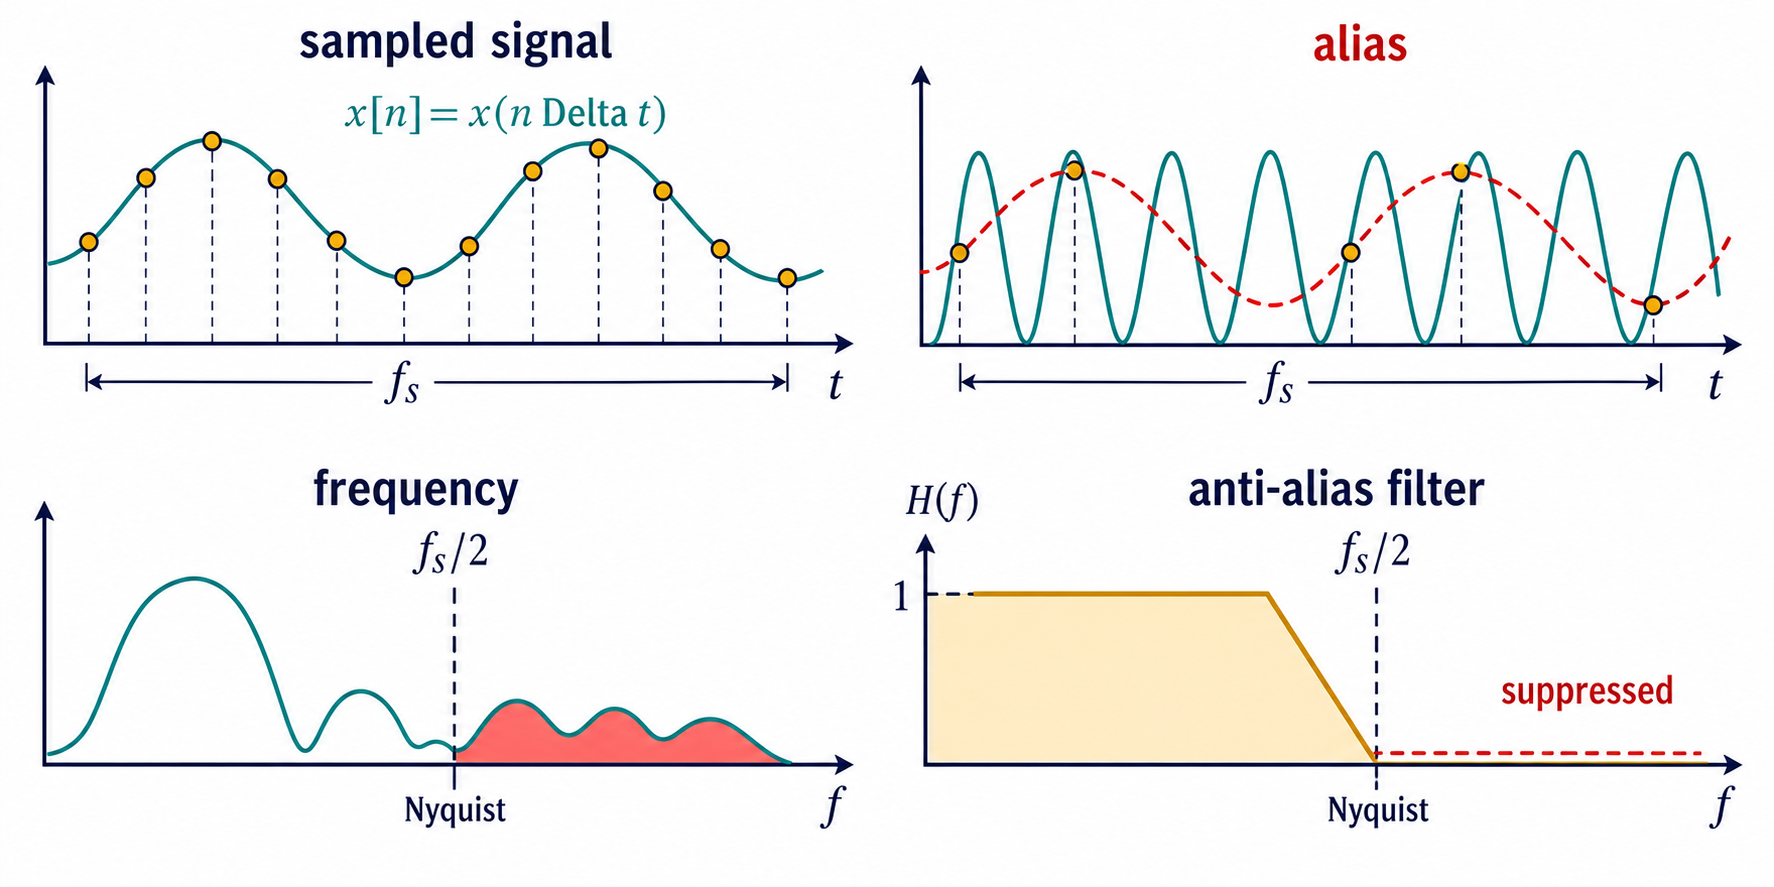
\includegraphics[width=0.96\linewidth]{imagegen-figures/ch12-sampling-aliasing-filters.png}
\caption{Sampling records a continuous signal only at discrete times. Frequencies above the Nyquist limit \(f_s/2\) can appear as lower-frequency aliases. An anti-alias low-pass filter suppresses frequencies above \(f_s/2\) before sampling so that the recorded sequence represents the intended band of the original signal.}
\label{fig:ch12-sampling-aliasing-filters}
\end{figure}

\paragraph{Formal setup.}
Let \(x:\mathbb{R}\to\mathbb{R}\) be a continuous-time signal. Sampling with interval \(\Delta t\) gives
\[
\boxed{x[n]=x(n\Delta t),\qquad f_s=\frac{1}{\Delta t}.}
\]
If \(x(t)=\cos(2\pi f_0t)\), then for any integer \(m\),
\[
\cos\left(2\pi (f_0+mf_s)n\Delta t\right)
=
\cos\left(2\pi f_0 n\Delta t+2\pi mn\right)
=
\cos\left(2\pi f_0 n\Delta t\right).
\]
Thus frequencies separated by integer multiples of \(f_s\) produce identical samples.

A signal is \emph{bandlimited} to \(B\) Hz if its Fourier transform is zero outside \([-B,B]\). The Nyquist-Shannon sampling theorem says, in one common form, that if \(x\) is bandlimited to \(B\) and
\[
f_s>2B,
\]
then \(x(t)\) can be reconstructed exactly from its samples using sinc interpolation:
\[
x(t)=\sum_{n=-\infty}^{\infty} x[n]\,
\operatorname{sinc}\left(\frac{t-n\Delta t}{\Delta t}\right),
\qquad
\operatorname{sinc}(u)=\frac{\sin(\pi u)}{\pi u}.
\]
The frequency \(f_s/2\) is the \emph{Nyquist frequency}. Before sampling, an \emph{anti-alias filter} removes frequencies above the Nyquist frequency.

\paragraph{Core intuition.}
Figure~\ref{fig:ch12-sampling-aliasing-filters} shows the main failure mode. If samples are dense compared with the signal's oscillation, the sample dots track the curve. If the signal oscillates too quickly, a slower curve can pass through the same sample dots. The discrete data cannot distinguish them.

In the frequency domain, sampling creates repeated copies of the original spectrum spaced by \(f_s\). If the original signal has frequency content above \(f_s/2\), those spectral copies overlap. That overlap is aliasing. A low-pass anti-alias filter removes high-frequency content before sampling so the copies do not collide.

Filters are operators that shape spectra. A filter with frequency response \(H(f)\) maps an input spectrum \(X(f)\) to
\[
Y(f)=H(f)X(f).
\]
A low-pass filter keeps slow components and suppresses rapid ones. A high-pass filter does the reverse. A band-pass filter keeps a chosen frequency range. In time, many filters are convolution operators; in frequency, they are multipliers.

Common misconceptions are costly in data analysis. First, increasing the number of plotted points after sampling does not undo aliasing. Interpolation can make a curve look smooth while preserving the wrong frequency. Second, Nyquist is about the highest frequency present in the signal before sampling, not the frequency that looks largest after sampling. Third, filters are not neutral preprocessing steps; they encode assumptions about which frequency content matters.

This section connects Chapter 12 back to practical measurement. It prepares digital signal processing, neural time-series analysis, imaging pipelines, audio models, discrete convolutions, and experimental design.

\paragraph{Main theorem: Nyquist sampling and aliasing.}
If a continuous-time signal is bandlimited to \(B\) Hz and sampled at rate \(f_s>2B\), then it is exactly determined by its samples. If frequency content above \(f_s/2\) is present, then distinct continuous frequencies can produce the same sample sequence, so aliasing is possible.

\emph{Proof sketch.}
The Fourier transform of a bandlimited signal occupies only \([-B,B]\). Sampling multiplies the signal by an impulse train in time. In the frequency domain, that multiplication creates shifted copies of the spectrum at multiples of \(f_s\). If \(f_s>2B\), the shifted copies do not overlap, so the original copy can be isolated by an ideal low-pass filter and transformed back to reconstruct \(x(t)\).

If \(f_s\leq 2B\), copies can overlap. The algebraic aliasing identity for sinusoids shows the ambiguity directly:
\[
\cos\left(2\pi (f_0+mf_s)n\Delta t\right)
=
\cos\left(2\pi f_0 n\Delta t\right).
\]
Two different continuous frequencies have the same samples. Once the samples are identical, no reconstruction method using only those samples can know which frequency generated them.

\paragraph{Worked examples.}
\emph{Small numerical example.} Suppose \(f_s=10\) Hz and \(\Delta t=0.1\) seconds. A 2 Hz cosine gives samples
\[
x_2[n]=\cos\left(2\pi\frac{2}{10}n\right)
=\cos(0.4\pi n).
\]
A 12 Hz cosine gives
\[
x_{12}[n]=\cos\left(2\pi\frac{12}{10}n\right)
=\cos(2.4\pi n)
=\cos(0.4\pi n+2\pi n)
=\cos(0.4\pi n).
\]
The two sample sequences are identical. At a 10 Hz sampling rate, 12 Hz aliases to 2 Hz.

\emph{ML/neuroscience example.} Suppose an EEG system samples at \(f_s=500\) Hz. The Nyquist frequency is \(250\) Hz. If muscle artifact or line-noise harmonics above \(250\) Hz enter the recording before digitization, they can alias into lower frequencies and contaminate the band used for analysis. An analog anti-alias filter before the digitizer is therefore part of the measurement model, not an optional cosmetic step.

\paragraph{ML/DL/neuroscience connections.}
In machine learning, downsampling images, audio, or time-series data without low-pass filtering can create aliases that a model may learn as spurious patterns. In deep learning, strided convolutions and pooling are discrete sampling operations; anti-aliasing layers reduce artifacts by filtering before subsampling. In neuroscience, spike binning, calcium imaging frame rates, EEG sampling rates, and local field potential preprocessing all depend on the same sampling theorem. The continuous signal \(x(t)\) becomes a recorded sequence \(x[n]\), the sampling rate \(f_s\) sets the recoverable frequency band, and the filter \(H(f)\) decides which parts of the spectrum survive.

\paragraph{Exercises.}
\begin{enumerate}[label=\textbf{12.4.\arabic*.}, leftmargin=*]
\item \textbf{Mechanical.} If \(\Delta t=0.002\) seconds, compute the sampling rate \(f_s\) and the Nyquist frequency.
\item \textbf{Proof or derivation.} Show that frequencies \(f_0\) and \(f_0+mf_s\), where \(m\) is an integer, produce identical samples for \(x(t)=\cos(2\pi f_0t)\).
\item \textbf{Numerical/computational.} With \(f_s=100\) Hz, compute the sampled sequences for 10 Hz and 110 Hz cosines for \(n=0,1,2,3,4\). Verify that they match.
\item \textbf{Interpretation.} A neural recording is sampled at 1000 Hz and then downsampled to 100 Hz. What must be true of the signal before downsampling to avoid aliasing?
\item \textbf{Debug the misconception.} A student says, "If a sampled plot looks smooth after interpolation, aliasing cannot have occurred." Explain why this is false.
\end{enumerate}

\paragraph{Closing bridge.}
This chapter turned functions into geometric objects, operators into maps between those objects, and Fourier analysis into a coordinate system built from oscillatory basis functions. Later chapters reuse this language whenever uncertainty, data, or dynamics are function-valued: probability densities are functions, expectations are integrals of functions, kernels compare or transform functions, PDEs use differential operators, CNNs learn convolutional operators, and neural field models evolve activity functions over space and time.

\clearpage
